\documentclass[11pt,letterpaper]{article}     % Tipo de documento y otras especificaciones
\usepackage[utf8]{inputenc}                   % Para escribir tildes y eñes
\usepackage[spanish]{babel}                   % Para que los títulos de figuras, tablas y otros estén en español
\usepackage[apaciteclassic]{apacite}
\usepackage{geometry}    
\usepackage{textcomp}
\geometry{left=25mm, right=25mm, top=25mm, bottom=25mm} % Tamaño del área de escritura de la página
\usepackage{amsmath}      % Los paquetes ams son desarrollados por la American Mathematical Society
\usepackage{amsfonts}     % y mejoran la escritura de fórmulas y símbolos matemáticos.
\usepackage{booktabs}
\usepackage{subfig}
\usepackage{amssymb}
\usepackage{graphicx}     % Para insertar gráficas
\usepackage{float}		% Para ubicar las tablas y figuras justo después del texto
\usepackage{pdfpages}
\batchmode
\usepackage{enumerate}
\usepackage{siunitx}
\pagestyle{plain} 
\usepackage{graphics}
\pagenumbering{arabic}
\usepackage{multicol}   % Para varias columnas
\usepackage{multirow}
\usepackage{color}%Paquete para colocar color al texto
%====================Español Venezolano Rápido============================
\renewcommand\tablename{Tabla}
\renewcommand\figurename{Figura}
%\renewcommand\prefacename{Prefacio}
\renewcommand\refname{REFERENCIAS}
%\renewcommand\bibname{REFERENCIAS}
\renewcommand\abstractname{Resumen}
%\renewcommand\chaptername{CAPÍTULO}
\renewcommand\appendixname{Apéndice}
\renewcommand\contentsname{ÍNDICE GENERAL}
\renewcommand\listfigurename{LISTA DE FIGURAS}
\renewcommand\listtablename{LISTA DE TABLAS}
\renewcommand\indexname{Índice Alfabético}
\renewcommand\partname{Parte}

%\renewcommand\enclname{Adjunto}
%\renewcommand\ccname{Copia a}
%\renewcommand\headtoname{A}
%\renewcommand\pagename{Página}
%\renewcommand\seename{véase}
%\renewcommand\alsoname{véase también}
%\renewcommand\proofname{Demostración}
%\renewcommand\glossaryname{Glosario}
%===================  Español venezolano =====================


\author{\\Raven Guillermo CI: 25.476.227\\Profesor: Crespo Jorge \vspace*{1in}}
\title{Universidad Central de Venezuela\\{ Facultad de Ingeniería\\Escuela de Ingeniería Eléctrica\\ Conversión Electromecánica de la energía\\\vspace*{1.5in} }Laboratorios 6 y 7\\MAQUINAS DE CORRIENTE CONTINUA\vspace*{1.35in}}
\date{Caracas, \today}

\begin{document}	% Inicio del documento
\maketitle							% Título
\newpage
\tableofcontents
\newpage
\section{Objetivos}
\begin{itemize}
	\item Estudiar los diferentes tipos de motores de corriente continua y sus
    aplicaciones en la industria.
	\item Modelar en régimen permanente una máquina de corriente continua.
	\item Determinar las curvas características más importantes de las máquinas de
    corriente continua.
    \item Estudiar los problemas asociados a la conmutación de una máquina de
    corriente continua.
\end{itemize}

\section{Lista de instrumentos}
\begin{table}[H]
	\caption{Lista de instrumentos de medición y componentes}
	\centering
	\begin{tabular}{|c|c|}
		\hline 
		Instrumento & Alcance ó especificaciones \\ \hline 
		Reostato &  (0-100) $\Omega$; 2.4 A \\  
		\hline 
		Reostato &  (0-33) $\Omega$; 4.2 A \\  
		\hline
		Voltímetros de bobina móvil y hierro móvil &  (0-150) V/ (0-15) V/(0-30) V/(0-300) V\\  
		\hline 
			Multímetro fluke & -\\  
		\hline 
		Resistencia de shunt & 40 A @ 60 mV\\  
		\hline
		Tacometro & -\\  
		\hline
		Amperímetro de bobina móvil y hierro móvil &(0-1.2) A/ (0-6) A/(0-30) A \\ 
		\hline
		Protecciones AC & 25 A; 380 V\\ 
		\hline
		Protecciones DC & -\\ 
		\hline
		Carga lineal & (200,400,600,800,1K)W  \\
        \hline
        \multirow{8}{3cm}{Motor sincrónico} & 3.5 KVA \\ 
        \cline{2-2}
        & 120/208 V \\
        \cline{2-2}
        & 16,8/9,7 A\\
        \cline{2-2}
        &1000 rpm\\
        \cline{2-2}
        &Iexc 3 A\\
        \cline{2-2}
        &Vexc 125 V\\
        \cline{2-2}
        & fp 0,9
        \\ \hline
        \multirow{5}{3cm}{Motor DC} & 115 V \\ 
        \cline{2-2}
        & 56A  \\
        \cline{2-2}
        & 1000 rpm\\
        \cline{2-2}
        &6,5 hp\\
        \cline{2-2}
        &carga 100\%\\
        \hline
        \multirow{5}{3cm}{Generador DC} & 3 KV\\ 
        \cline{2-2}
        & 125 V \\
        \cline{2-2}
        &26,5 A\\
        \cline{2-2}
        & 1000 rpm\\
        \hline

        
	\end{tabular} 
\end{table}
\section{Condiciones de ensayo}
Estas son las precauciones y normativas necesarias para realizar el laboratorio de forma segura y efectiva: 
\begin{itemize}
    \item \textbf{Respecto a la medición de la curva en vacío:} La máquina a la que se le hará la prueba deberá estar conectada como generador. Dado que tiene que girar a velocidad constante, se utilizara algún mecanismo externo que brinde tales características. 
    
    Este sera un motor sincrónico o una turbina. En el caso de emplearse un motor sincrónico el campo deberá activarse al alcanzar una velocidad constante.
    \item \textbf{Respecto a la medición de resistencias:} Se trabajara asegurándose que la corriente máxima alcanzada en $I_{f}$ ó $I_{a}$ sea menor o igual al 10 \% de la corriente nominal. La resistencia obtenida mediante la pendiente de la recta debe ajustarse de acuerdo a la temperatura.
    \item \textbf{Respecto a la medición de la característica de regulación:} Se debe mantener $U_{c}$ (tensión en los bornes) en su valor nominal y a velocidad nominal. 
    \item  \textbf{Respecto a la medición del porcentaje de regulación:} Se debe comenzar a medir la tensión en los bornes comenzando desde el valor a plena carga.
    \item \textbf{Respecto a la medición de la curva de carga:} Se debe medir a velocidad constante.
    \item \textbf{Respecto a la medición de la curva electromecánica de par:} Se deben mantener $U_{c}$ constante y $I_{exc}$.
    \item \textbf{Respecto a la medición de la curva electromecánica de velocidad:} La tensión en los bornes (Uc) deberá mantenerse a su valor nominal y la corriente de excitación también.
    \item  \textbf{Respecto a la medición del porcentaje de regulación de velocidad:} Se comenzara a medir desde la carga nominal ($I_{a}$ nominal y N nominal).
    \item  \textbf{Respecto a la medición de la curva de regulación de velocidad:} Sin importar si se utiliza el método de control por corriente de campo ó el método de ajuste de tensión en los terminales de armadura. Es necesario mantener en ambos el par constante, aunque en el primero la corriente de excitación es constante, en cambio en el segundo sera constante la tensión en los bornes.
    \item  \textbf{Respecto a la medición de la curva de regulación de par:} Sin importar si se utiliza el método de control por corriente de campo ó el método de ajuste de tensión en los terminales de armadura. Es necesario mantener en ambos la velocidad constante, aunque en el primero la corriente de excitación es constante, en cambio en el segundo sera constante la tensión en los bornes.  
    \item \textbf{Respecto a la  vestimenta:} No usar franelas o camisas manga larga, llevar zapatos de goma y pantalones. No usar collares ni pulseras de metal.
    \item \textbf{Previo a las pruebas:} Hacer primero el montaje antes de energizar, al culminarlo preguntar al profesor si las conexiones son correctas para proceder con las pruebas.
    \item \textbf{Respecto a la comunicación:} Mantener informado sobre cualquier cambio en el montaje al compañero de laboratorio y por sobre todo informar si el circuito se encuentra energizado o no.
	\item \textbf{Respecto a las curvas observadas:} No aceptar como adecuada una curva que este llena de ruido, ya que se puede deber a que algún elemento puede estar actuando como antena, esto originara incertidumbre en los resultados.
	\item \textbf{Respecto al numero de mediciones:}
	Realizar al menos 5 mediciones para condiciones distintas.
	\item \textbf{Respecto a la elección de componentes y las conexiones:} Evitar los componentes que puedan funcionar como antenas (como resistencias de shunt de tipo mariposa u algún otro que se encuentre muy expuesto) y cuidar los contactos de cada conexión.
    \item \textbf{Respecto a la manipulación:} En caso de maniobrar el circuito energizado manipular con la mano derecha, buscando mayores probabilidades de sobrevivir en caso de un accidente eléctrico.
\end{itemize}
\section{Procedimiento}
\subsection{Características internas}
\subsubsection{Caídas internas}
\begin{enumerate}
    \item Lo primero sera, hallar las resistencias internas de campo y armadura por lo que se realizaran las conexiones como en la Figura \ref{fig:diagMedRes}.
    \item Se conectara unicamente el lado de campo con una fuente DC (a una fracción del valor nominal).
    \item Manteniendo la tensión $V_{f}$ fija y variando el reostato en pasos equidistantes se tomara nota de los valores de tensión y corriente. Se tomaran al menos 4 mediciones.
    \item Se desconectara la alimentación del lado de campo y se conectara la fuente del lado serie repitiendo así los pasos previos.
    \item Se desconectara la alimentación del lado serie y se conectara la fuente del lado de armadura a tensión por debajo del valor nominal.
    \item Manteniendo la tensión $V_{a}$ fija y desplazando la cuchilla de arranque en pasos equidistantes se tomara nota de los valores de tensión en los bornes y la tensión en la resistencia de shunt. Se tomaran al menos 5 mediciones.
    
    \item Se desconectara la alimentación del lado de armadura y se des-energizara el circuito.
\end{enumerate}
\subsubsection{Curva de saturación ó vacío}
\begin{enumerate}
	\item Se armara el esquema de conexiones conectando el motor DC como generador de acuerdo a la figura \ref{fig:diagMedCurvaCaracteristica}.
	\item Se encenderá el generador sincrónico y solo cuando alcance una velocidad constante se accionara el campo mediante las protecciones DC.
	\item Manteniendo la velocidad del eje a su valor nominal se variara el reostato del lado de campo de forma que los datos sean tomados en espacios apropiados que permitirán una exactitud de la curva graficada entre nula excitación y 125 \% de la tensión nominal ($U_{nom}$), en la parte lineal de la curva con incrementos de 20 \% de $U_{nom}$ y pasos del 10 \% de $U_{nom}$,
	alrededor del codo de saturación que suele estar entre el 80 \% y el 110 \% de la $U_{nom}$.  
	\item Se repetirá el proceso del punto previo; pero desde el ultimo punto alcanzado hasta el valor mínimo, respetando en lo posible que los pasos sean iguales.
\end{enumerate}
\subsection{Características externas}
\subsubsection{Característica de regulación y porcentaje de regulación}
\begin{enumerate}
    \item Se realiza la conexión de la Figura \ref{fig:diagGeneradorIndependiente} de generador independiente.
    \item Empleando el tacometro se verifica velocidad nominal en el generador.
    \item Se ajusta $U_{c}$ inicialmente sin carga hasta alcanzar $U_{nom}$ con $I_{ext}$, una vez alcanzado $U_{nom}$ se registra el valor.
    \item Se conecta carga al sistema, generando un cambio en los valores de $U_{c}$ e $I_a$.
    \item Se ajusta $U_{c}$ con $I_{ext}$ hasta alcanzar valores nominales. Se registra el valor de $I_{ext}$ e $I_a$.
    \item Se varía la carga y se repite hasta llegar a valores nominales.
    \item Una vez registrado el ultimo valor se verifica que se encuentre en $U_{nom}$ e $I_{anom}$ en caso que sean diferentes se ajustarán a valores nominales, una vez verificado se desconectará la carga de forma gradual hasta retirarla completamente, luego se registra e valor de $U$ sin carga. 
\end{enumerate}
\subsection{Motor independiente}
\subsubsection{Curva de velocidad en función de la corriente de armadura}
\begin{enumerate}
    \item Se realiza la conexión de la fig \ref{fig:diagMotorIndependiente} de motor independiente.
    \item Se realiza la medición de la curva electromecánica de velocidad manteniendo Uc constante e $I_{ext}$ constante.
    \item Se anotan las mediciones de $I_a$ y de la velocidad.
    \item Se varia Rs, por lo que varia $I_a$ directamente. Se anotan los valores y se repite hasta tener varias mediciones.
\end{enumerate}
\subsubsection{Determinar el PRN\%}
\begin{enumerate}
    \item Se toman las medidas a $I_a$ nominal y N nominal con tensión de armadura e Iexc constante.
    \item Se eleva la carga lineal hasta el valor nominal del motor. Se registran los datos
    \item Se quita la carga y se toman los datos.
\end{enumerate}
\subsection{Pérdidas en vacío}
\begin{enumerate}
    \item Para calcular las perdidas en el vacío se deben realizar medidas en dos velocidades distintas anotando los valores de corriente y tensión asociados.
\end{enumerate}
\section{Diagramas}
\begin{figure}[H]
    \centering
    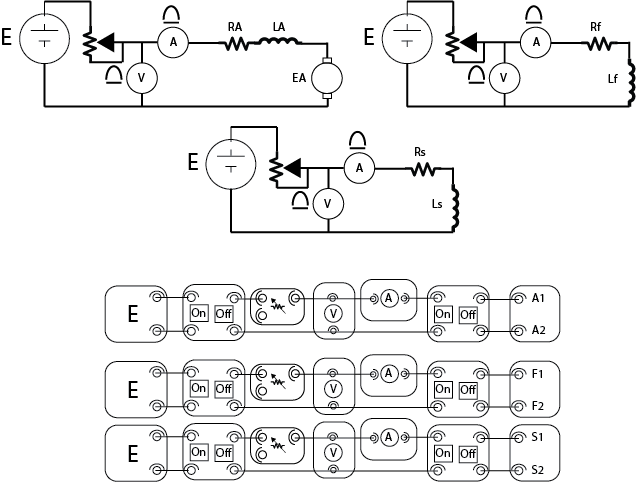
\includegraphics[scale=0.5]{./recursos-Lab6/diagMedRes.png}
    \caption{Diagrama de conexión pruebas de resistencias internas}
    \label{fig:diagMedRes}
\end{figure}
\begin{figure}[H]
    \centering
    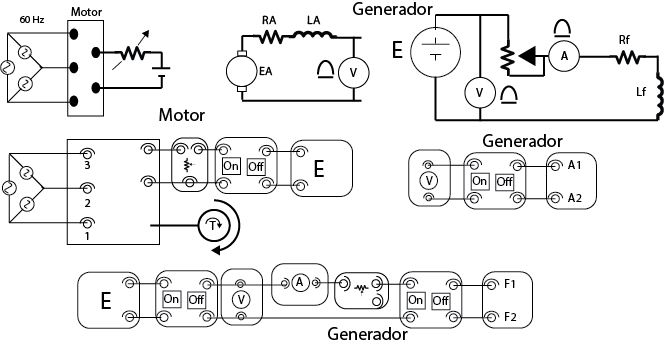
\includegraphics[scale=0.5]{./recursos-Lab6/diagMedCurvaVacio.png}
    \caption{Diagrama de conexión pruebas de Prueba curva de vacio}
    \label{fig:diagMedCurvaCaracteristica}
\end{figure}
\begin{figure}[H]
    \centering
    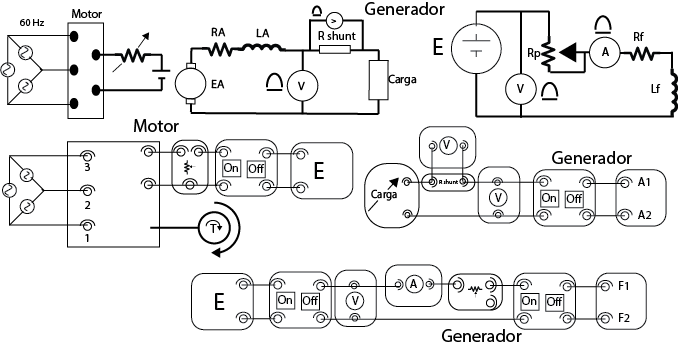
\includegraphics[scale=0.5]{./recursos-Lab6/diagGeneradorIndependiente.png}
    \caption{Diagrama de conexión de generador independiente}
    \label{fig:diagGeneradorIndependiente}
\end{figure}
\begin{figure}[H]
    \centering
    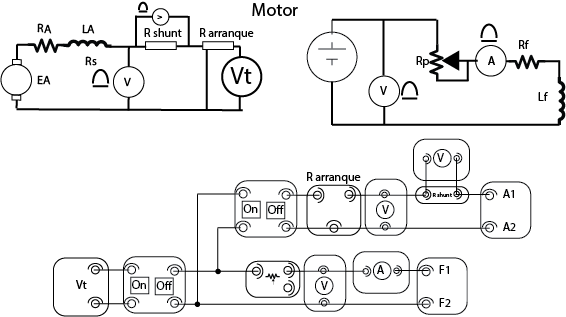
\includegraphics[scale=0.5]{./recursos-Lab6/diagMotorIndependient.png}
    \caption{Diagrama de conexión de motor independiente}
    \label{fig:diagMotorIndependiente}
\end{figure}
\section{Cálculos preliminares}
\subsection{Características internas}
\subsubsection{Resistencia interna }
De acuerdo al diagrama de la figura \ref{fig:diagMedRes}, se espera una curva característica de tensión vs corriente para el lado de campo con una forma similar al de la figura \ref{fig:curvaCaractPreVILadoCampo} y en el lado de armadura su forma se asemejara a la figura \ref{fig:curvaCaractPreVILadoArmadura}.
\begin{figure}[H]
    \centering
    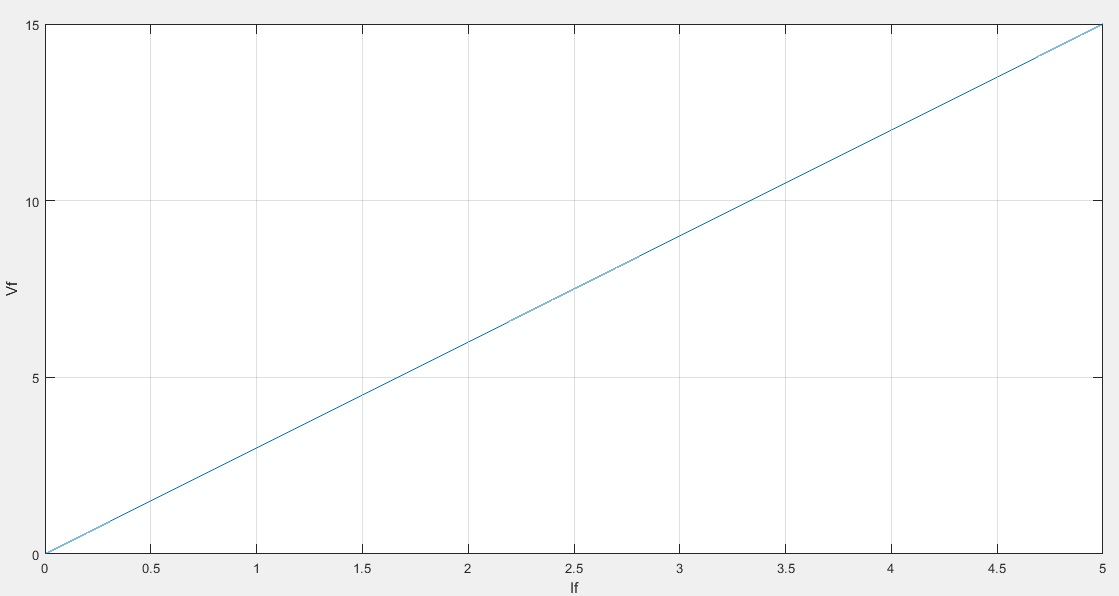
\includegraphics[scale=0.5]{./recursos-Lab6/curvaCaractPreVILadoCampo.jpg}
    \caption{Curva característica esperada V vs $I_{f}$}
    \label{fig:curvaCaractPreVILadoCampo}
\end{figure}
La pendiente de la curva previa proporcionara el valor de la resistencia de campo.
\begin{figure}[H]
    \centering
    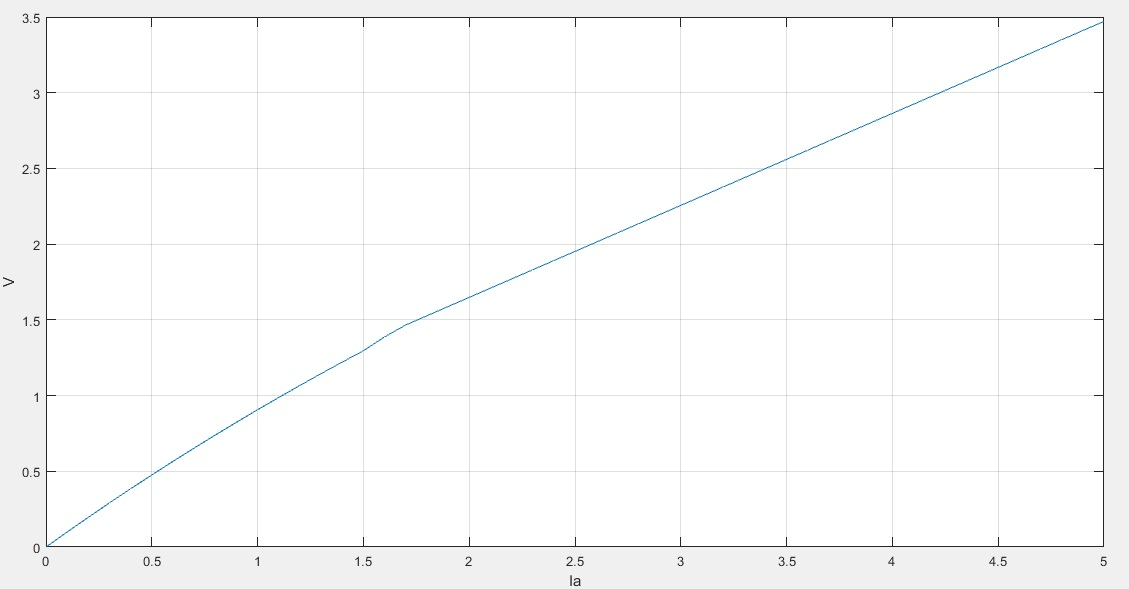
\includegraphics[scale=0.5]{./recursos-Lab6/curvaCaractPreVILadoArmadura.jpg}
    \caption{Curva característica esperada V vs $I_{a}$}
    \label{fig:curvaCaractPreVILadoArmadura}
\end{figure} 
Como se puede observar en la figura \ref{fig:curvaCaractPreVILadoArmadura} a diferencia de la figura \ref{fig:curvaCaractPreVILadoCampo} no es una recta completamente. Al inicio de la curva se espera un comportamiento no lineal debido a la resistencia de las escobillas; Aunque desde cierto punto se vuelve lineal debido a que el ya mencionado efecto es despreciable, por lo que la pendiente de la zona lineal corresponde con el valor de la resistencia de armadura. 
\section{Resultados}
\subsection{Características internas}
\subsubsection{Resistencia de campo}
Se realizaron las siguientes mediciones:
\begin{table}[H]
	\centering
	\caption{Valores obtenidos por método de voltímetro-amperímetro para Rf}
	\label{VoltimetroAmperimetroRf}
	\begin{tabular}{|c|c|}
		\hline
		\textbf{Tensión {[}V{]}} & \textbf{Corriente {[}A{]}} \\ \hline
		6,0 $\pm$ 0,1            & 0,12 $\pm$ 0,02            \\ \hline
		7,0 $\pm$ 0,1            & 0,14 $\pm$ 0,02            \\ \hline
		8,0 $\pm$ 0,1            & 0,16 $\pm$ 0,02            \\ \hline
		8,5 $\pm$ 0,1            & 0,18 $\pm$ 0,02            \\ \hline
		9,0 $\pm$ 0,1            & 0,2 $\pm$ 0,02             \\ \hline
	\end{tabular}
\end{table}
Utilizando los valores del cuadro \ref{VoltimetroAmperimetroRf} se linealizó mediante mínimos cuadrados y se obtuvo lo siguiente:
\begin{figure}[H]
	\centering
	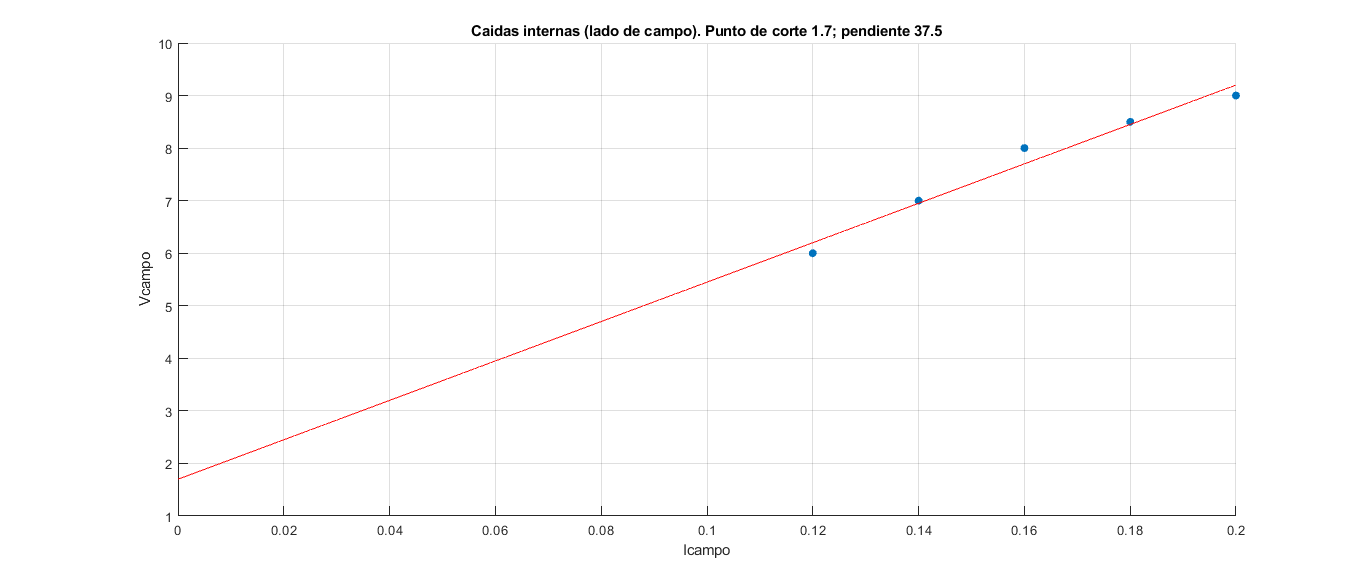
\includegraphics[scale=0.5]{./recursos-Lab6/caidasInternasCAMPO.png}
	\caption{Recta obtenida por regresión lineal que corresponde con la resistencia de campo}
	\label{fig:rectaResistenciaCampo}
\end{figure}
Para calcular la incertidumbre asociada a la pendiente hallada se determino la desviación estandar:
\begin{equation}
	\sigma = \sqrt{\frac{\sum_{i=1}^{N}(y_{i}-m\cdot x_{i}-b)^{2}}{N-2}} \label{desvEstandar}
\end{equation}
Donde:\\
N: numero de datos\\
b: Punto de corte obtenido\\
m: Pendiente obtenida\\
$y_{i}$: Datos del eje y\\
$x_{i}$: Datos del eje x

Utilizando la desviación se calcula incertidumbre de la pendiente mediante la siguiente ecuación:
\begin{equation}
	\Delta m = \sigma \sqrt{\frac{N}{N\sum_{i=1}^{N}x_{i}^{2}-\left(\sum_{i=1}^{N}x_{i}\right)^{2}}} \label{incertiPendiente}
\end{equation}
Por lo tanto la resistencia de campo medida sera: $R_{f(medida)}$ = 37,50 $\pm$ 0,29 $\Omega$. No obstante se requiere ajustar el valor respecto a la temperatura empleando la siguiente expresión:
\begin{align}
	R_{f} = R_{(medida)} \frac{T_{r}+T_{k}}{T_{m}+T_{k}} \label{ajusteTemp}
\end{align}
donde:\\
$T_{k}$ : 234.5 \textdegree C (cobre).\\
$T_{m}$ : Temperatura a la cual se midió la resistencia, 25 \textdegree C.\\
$T_{r}$ : Es la temperatura de referencia en \textdegree C (75 \textdegree C).\\
Entonces: $R_{f(ajustada)}$ = 44,73 $\pm$ 0,29 $\Omega$.
\subsubsection{Resistencia de armadura y tensión en escobillas}
Se realizaron las siguientes mediciones:
\begin{table}[H]
	\centering
	\caption{Valores obtenidos por método de voltímetro-amperímetro para Ra}
	\label{VoltimetroAmperimetroRA}
	\begin{tabular}{|c|c|}
		\hline
		\textbf{Tensión {[}V{]}} & \textbf{Corriente {[}A{]}} \\ \hline
		0,869 $\pm$ 0,001            & 2,5 $\pm$ 0,5            \\ \hline
		1,356 $\pm$ 0,001            & 4,0 $\pm$ 0,5            \\ \hline
		1,563 $\pm$ 0,001            & 5,0 $\pm$ 0,5            \\ \hline
		1,751 $\pm$ 0,001            & 5,5 $\pm$ 0,5            \\ \hline
		2,220 $\pm$ 0,001            & 7,5 $\pm$ 0,5             \\ \hline
		2,737 $\pm$ 0,001            & 10,0 $\pm$ 0,5             \\ \hline
	\end{tabular}
\end{table}
Empleando los valores del cuadro \ref{VoltimetroAmperimetroRA} se linealizó mediante mínimos cuadrados y se obtuvo lo siguiente:
\begin{figure}[H]
	\centering
	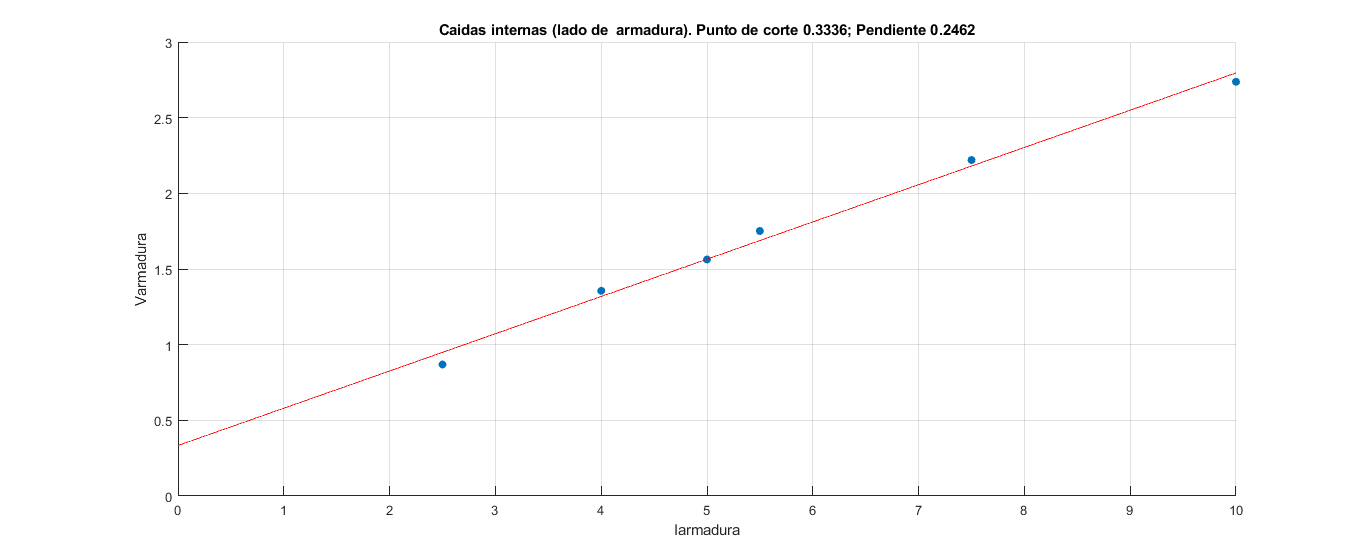
\includegraphics[scale=0.5]{./recursos-Lab6/caidasInternasARMADURA.png}
	\caption{Recta obtenida por regresión lineal que corresponde con la resistencia de armadura y tensión en escobillas}
	\label{fig:rectaResistenciaArmadura}
\end{figure}
Utilizando los datos obtenidos de la recta que corresponden con la resistencia de armadura y las ecuaciones \ref{desvEstandar} y \ref{incertiPendiente} se obtuvo que la resistencia de armadura medida es igual a: $R_{a(medida)}$ = = 0,2462 $\pm$ 0,0081 $\Omega$. No obstante se requiere ajustar el valor respecto a la temperatura usando la ecuación \ref{ajusteTemp}, de esta forma la resistencia de armadura real sera: $R_{a(ajustada)}$ = 0,2936 $\pm$ 0,0081 $\Omega$.

Por otro lado la tensión en las escobillas corresponde con el punto de corte con el eje y, la incertidumbre del mismo se calcula con:
\begin{equation}
	\Delta V_{esc} = \sigma \sqrt{\frac{\sum_{i=1}^{N}x_{i}^{2}}{N\sum_{i=1}^{N}x_{i}^{2}-\left(\sum_{i=1}^{N}x_{i}\right)^{2}}}
\end{equation}
Entonces dicha tensión sera: $V_{esc}$ = 0,3336 $\pm$ 0,0195 V. De acuerdo con IEC 34-2 e IEEE Std 113-1985 las escobillas del motor deben ser del tipo metal-grafito, con shunt debido a su tensión reducida. 
\subsubsection{Modelo Obtenido}
%% Enderson haz un diagrama circuital con conexión independiente donde le coloques el valor de las resistencias obtenidas con sus incertidumbres y la tensión en las escobillas obtenida
\begin{figure}[H]
	\centering
	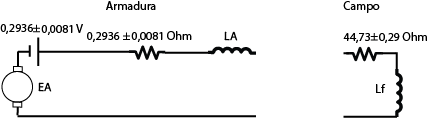
\includegraphics[scale=0.9]{./recursos-Lab6/diagModeloObtenido.png}
	\caption{Modelo que invluye valores obtenidos}
	\label{fig:modObtenido}
\end{figure}
\subsubsection{Resistencia serie}
Se realizaron las siguientes mediciones:
\begin{table}[H]
	\centering
	\caption{Valores obtenidos por método de voltímetro-amperímetro para Rs}
	\label{VoltimetroAmperimetroRs}
	\begin{tabular}{|c|c|}
		\hline
		\textbf{Tensión {[}mV{]}} & \textbf{Corriente {[}A{]}} \\ \hline
		7,3 $\pm$ 0,1            & 0,44 $\pm$ 0,02            \\ \hline
		8,5 $\pm$ 0,1            & 0,52 $\pm$ 0,02            \\ \hline
		9,0 $\pm$ 0,1            & 0,54 $\pm$ 0,02            \\ \hline
		10,0 $\pm$ 0,1            & 0,60 $\pm$ 0,02            \\ \hline
		11,4 $\pm$ 0,1            & 0,70 $\pm$ 0,02             \\ \hline
		13,6 $\pm$ 0,1            & 1,00 $\pm$ 0,02             \\ \hline
	\end{tabular}
\end{table}
Utilizando los valores del cuadro \ref{VoltimetroAmperimetroRs} se linealizó mediante mínimos cuadrados y se obtuvo lo siguiente:
\begin{figure}[H]
	\centering
	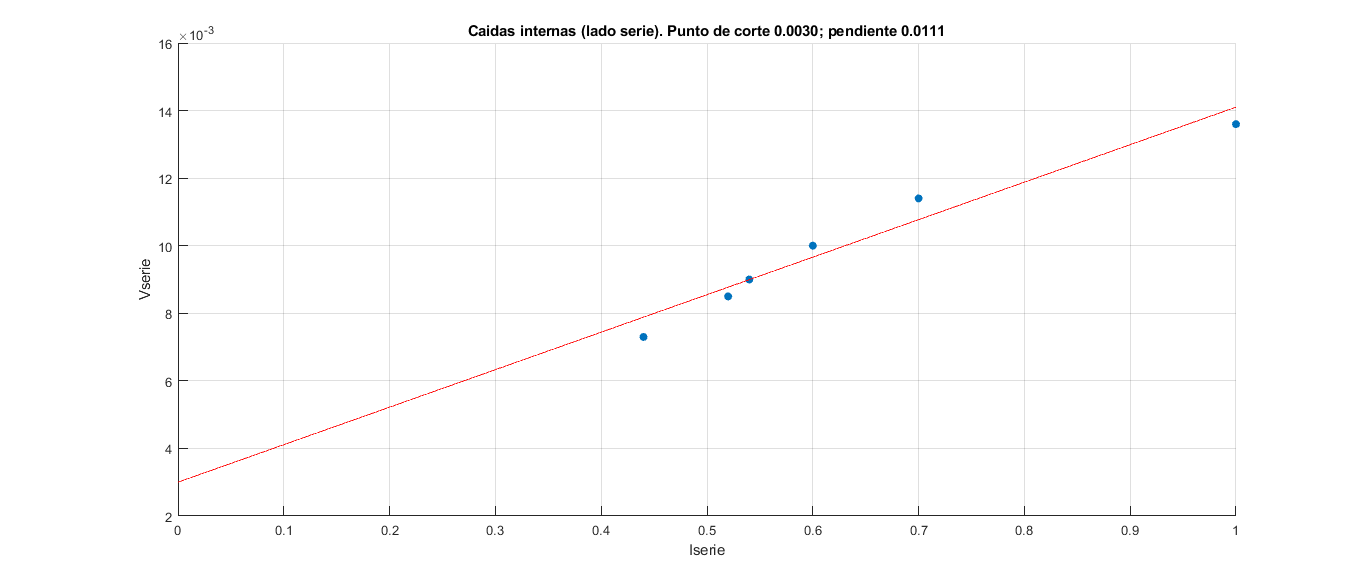
\includegraphics[scale=0.5]{./recursos-Lab6/caidasInternasSERIE.png}
	\caption{Recta obtenida por regresión lineal que corresponde con la resistencia serie}
	\label{fig:rectaResistenciaSerie}
\end{figure}
Empleando los datos obtenidos de la recta que corresponden con la resistencia serie y las ecuaciones \ref{desvEstandar} y \ref{incertiPendiente} se obtuvo que la resistencia en serie es igual a: $R_{s}$ = 11,05 $\pm$ 0,35 m$\Omega$.  No obstante se requiere ajustar el valor respecto a la temperatura usando la ecuación \ref{ajusteTemp}, de esta forma la resistencia serie real sera: $R_{s(ajustada)}$ = 13,18 $\pm$ 0,35 m$\Omega$.
\subsubsection{Curva de vacío}
Se realizaron mediciones de corriente y tensión a una velocidad constante de 1140 $\pm$ 2 rpm.
\begin{table}[H]
	\centering
	\caption{Meciciones de tensión de vacío y corriente de campo}
	\label{MedCurvaVacio}
	\begin{tabular}{|c|c|c|c|}
		\hline
		\multicolumn{2}{|c|}{Elevando}                        & \multicolumn{2}{c|}{Reduciendo}                       \\ \hline
		\textbf{$U_{0}$ {[}V{]}} & \textbf{$I_{exc}$ {[}A{]}} & \textbf{$U_{0}$ {[}V{]}} & \textbf{$I_{exc}$ {[}A{]}} \\ \hline
		60 $\pm$ 1               & 0,54 $\pm$ 0,02            & 109 $\pm$ 1              & 0,8 $\pm$ 0,1              \\ \hline
		74 $\pm$ 1               & 0,66 $\pm$ 0,02            & 90 $\pm$ 1               & 0,7 $\pm$ 0,1              \\ \hline
		89 $\pm$ 1               & 0,82 $\pm$ 0,02            & 80 $\pm$ 1               & 0,62 $\pm$ 0,02            \\ \hline
		107 $\pm$ 1              & 1,00 $\pm$ 0,02            & 73 $\pm$ 1               & 0,54 $\pm$ 0,02            \\ \hline
		132 $\pm$ 1              & 1,3 $\pm$ 0,1              & -                        & -                          \\ \hline
	\end{tabular}
\end{table}
Con los valores obtenidos en el cuadro \ref{MedCurvaVacio} se empleo la función polyfit(x,y,n) (n es el orden del polinomio) de Matlab con el fin de obtener un polinomio que se ajuste a los datos. Y se evaluó el polinomio mediante polyval(), para posteriormente obtener las siguientes curvas:
\begin{figure}[H]
	\centering
	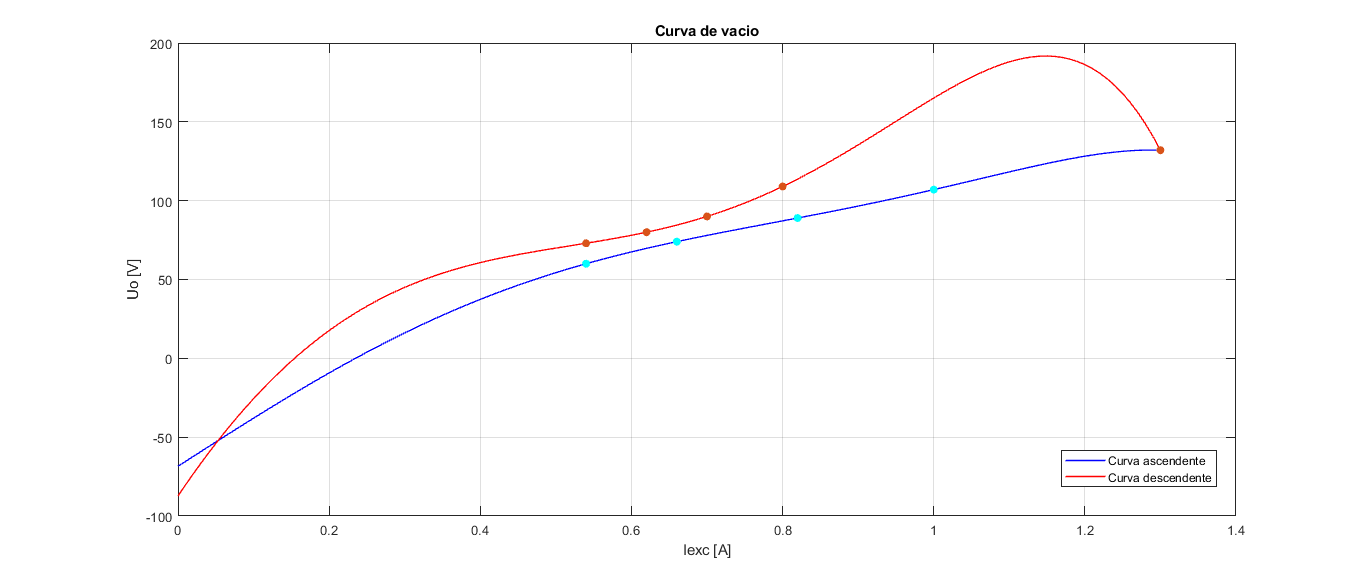
\includegraphics[scale=0.5]{./recursos-Lab6/curvaDeVacioExp.png}
	\caption{Curvas de vacío experimentales}
	\label{fig:curvaDeVacioExp}
\end{figure}
\subsection{Características externas (Funcionamiento como generador)}
\subsubsection{Curva característica de regulación}
Se agrego carga al generador y se ajusto el reostato del lado de campo, con el fin de mantener la velocidad nominal. Se obtuvieron los siguientes resultados:
\begin{table}[H]
	\centering
	\caption{Mediciones del efecto de la carga en la corriente de excitación}
	\label{MedCurvaCaractReg}
	\begin{tabular}{|c|c|}
		\hline
		\multicolumn{2}{|c|}{\textbf{$N_{nominal}$ = 1000 $\pm$ 2 {[}rpm{]}}} \\ \hline
		\textbf{$I_{exc}$ {[}A{]}}   & \textbf{$I_{a}$ {[}A{]}}               \\ \hline
		1,2 $\pm$ 0,1                & 0 (sin carga)                          \\ \hline
		1,3 $\pm$ 0,1                & 8,0 $\pm$ 0,5                          \\ \hline
		1,3 $\pm$ 0,1                & 16,0 $\pm$ 0,5                         \\ \hline
		1,1 $\pm$ 0,1                & 3,5 $\pm$ 0,5 (disminuyendo la carga)  \\ \hline
	\end{tabular}
\end{table}
Utilizando los datos obtenidos en el cuadro \ref{MedCurvaCaractReg}, a excepción punto obtenido al disminuir la carga es posible hallar un polinomio que se ajuste a los datos mediante matlab. En la Figura \ref{fig:curvaCaractReg} se observa el comportamiento del campo respecto a distintas cargas.
\begin{figure}[H]
	\centering
	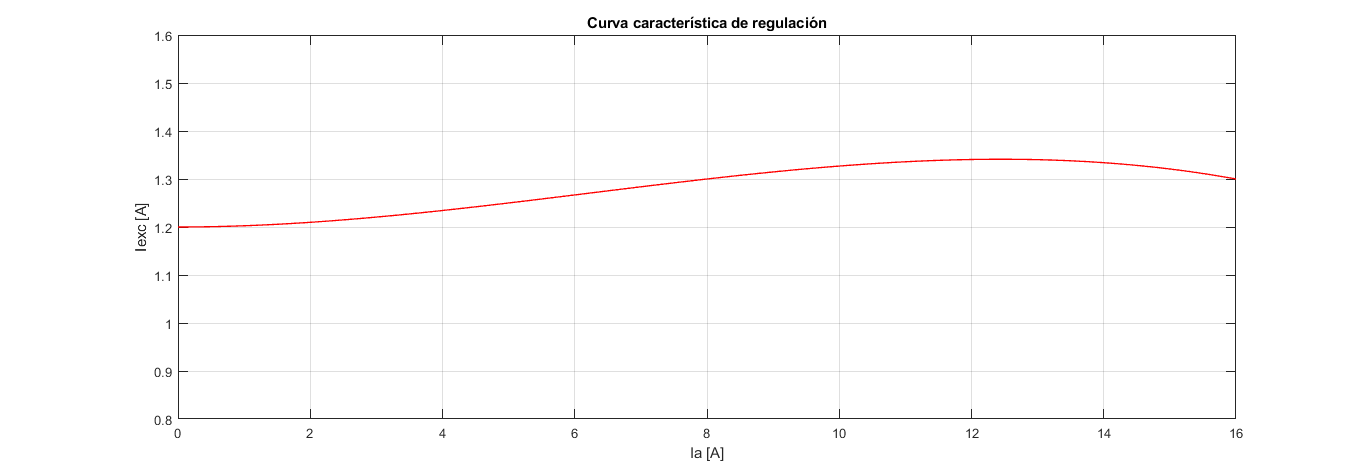
\includegraphics[scale=0.5]{./recursos-Lab6/curvaCaractRegulacion.png}
	\caption{Curvas característica de regulación experimental}
	\label{fig:curvaCaractReg}
\end{figure}
\subsubsection{Porcentaje de regulación}
Se midió la tensión a plena carga y luego sin carga. Se obtuvieron los siguientes resultados:
\begin{table}[H]
	\centering
	\caption{Mediciones para el porcentaje de regulación}
	\label{MedPReg}
	\begin{tabular}{|c|c|}
		\hline
		\textbf{$U_{pc}$ {[}V{]}} & \textbf{$U_{sc}$ {[}V{]}} \\ \hline
		125 $\pm$ 1               & 132 $\pm$ 1               \\ \hline
	\end{tabular}
\end{table}
Se sabe que el porcentaje de regulación de un generador DC viene dado por:
\begin{align}
	\%Reg = \frac{V_{sc}-V_{pc}}{V_{pc}}100\%\\
	\Delta \%Reg = \frac{100}{V_{pc}}\Delta V_{sc} + \frac{V_{sc}}{V_ {pc}^{2}}\Delta V_{pc}
\end{align}
Por medio de las dos ecuaciones previas se obtiene que la regulación es: \%Reg = 5.6 $\pm$ 0.8
\subsubsection{Curva de carga}
Se midió la capacidad del generador para mantener la tensión nominal a distintas cargas (Ver cuadro \ref{MedCurvaCarga}). 
\begin{table}[H]
	\centering
	\caption{Mediciones del efecto de carga en la tensión del generador}
	\label{MedCurvaCarga}
	\begin{tabular}{|c|c|}
		\hline
		\multicolumn{2}{|c|}{\textbf{$U_{c}$ =$U_{nominal}$ = 124 $\pm$ 1}} \\ \hline
		\textbf{$U_{c}$ {[}V{]}}         & \textbf{$I_{a}$ {[}A{]}}         \\ \hline
		120 $\pm$ 1                      & 3,0 $\pm$ 0,5                    \\ \hline
		119 $\pm$ 1                      & 7,5 $\pm$ 0,5                    \\ \hline
		118$\pm$ 1                       & 11,0 $\pm$ 0,5                   \\ \hline
		117$\pm$ 1                       & 15,0 $\pm$ 0,5                   \\ \hline
		116 $\pm$ 1                      & 18,0 $\pm$ 0,5                   \\ \hline
	\end{tabular}
\end{table}
Con los datos obtenidos en el cuadro \ref{MedCurvaCarga}, se hallo la curva presente en la Figura \ref{fig:CurvaDeCarga}. Dicha curva demuestra el efecto de la regulación para distintas cargas.
\begin{figure}[H]
	\centering
	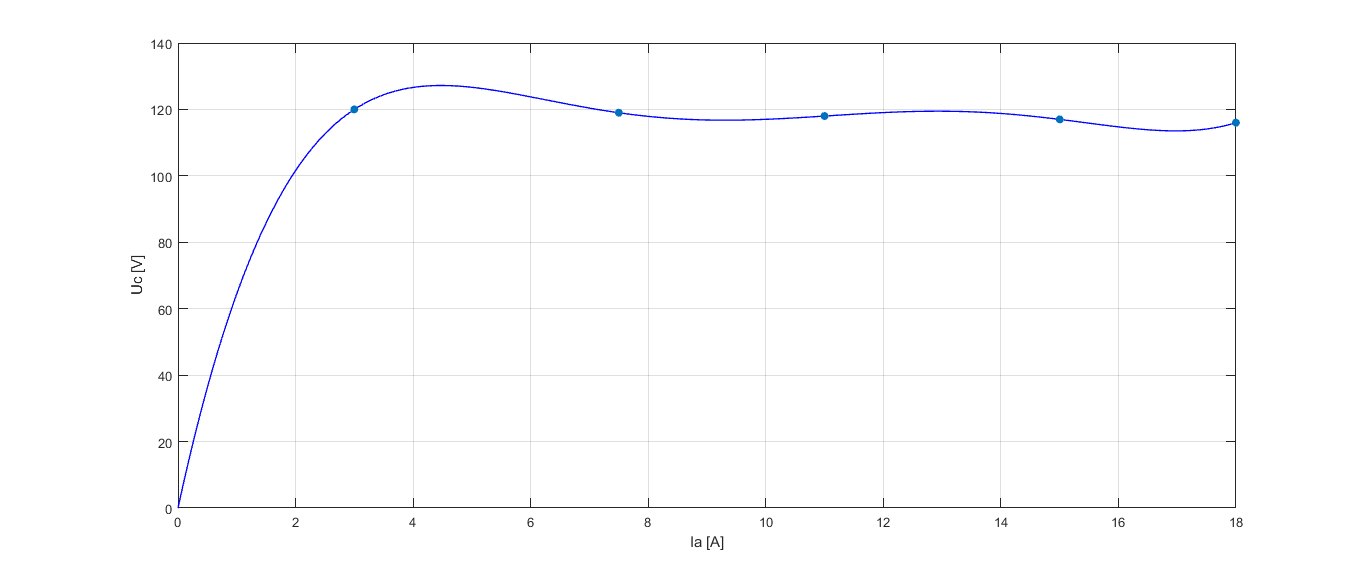
\includegraphics[scale=0.5]{./recursos-Lab6/CurvaDeCarga.png}
	\caption{Curvas de carga experimental}
	\label{fig:CurvaDeCarga}
\end{figure}
\subsection{Características externas (Funcionamiento como motor)}
	Se realiza la medición de la velocidad y la corriente de armadura empleando un rshunt, variando la carga y manteniendo fija la corriente de campo en 1,4 $\pm0,1$ A y la tensión nominal en 115V $\pm1$.\\
	
		La rshunt utilizada es de 40A@60mV, los valores de tensión obtenidos al estar en la escala de mV se multiplican por un factor de 4/6 para obtener la corriente que por ella circula.\\
		
		Sabemos que:
		
		\begin{equation}
			\tau_{ind}\cdot W_m = E_a*I_a 
			\label{ec.power}
		\end{equation}
		
		En la Figura \ref{fig:modObtenido} tenemos los parametros internos obtenidos previamente, Al despejar $\tau_{ind}$ de la ecuación \ref{ec.power} y encontrando el valor de Ea obtenemos:
		
		\begin{equation}
			\tau_{ind}=\frac{U_n\cdot I_a-I_a^2\cdot R_a}{W_m}
		\end{equation}
		
		\begin{equation}
		\Delta \tau_{ind}=	\frac{\Delta Wn {\left({Ia}^2  Ra-Ia Un\right)}}{Wn^{2}}+\frac{Ia \Delta Un}{Wn}+\frac{ \Delta Ia {\left({Un}-2 {Ia} {Ra}\right)}}{{Wn}}-\frac{{Ia}^2 {\Delta Ra}}{Wn}
		\end{equation}
		
		Con las ecuaciones planteadas y datos obtenidos en el labotarorio se presenta el siguiente cuadro:
	\begin{table}[H]
		\centering
			\caption{Mediciones del efecto de la carga en la tensión del motor y medición indirecta de la corriente de armadura}
		\begin{tabular}{|c|c|c|c|c|}
			\hline
			Vshunt (mV) & N(rpm) & Carga (W) &Ia(A)& Tind\\ \hline
			11,8 +- 0,1 & 1010 +- 2 & 200 & 7,87 +- 0,067&8.39 +- 0.124\\ \hline
			13,5 +- 0,1 & 1008 +- 2 & 400 & 9,00 +- 0,067&9.58+-0.131\\ \hline
			15,8 +- 0,1 & 1004 +- 2 & 600 & 10,53 +- 0,067&11.2+-0.14\\ \hline
			17 ,0 +- 0,1 & 992 +- 2 & 800 & 11,33 +- 0,067& 12.2+-0.145\\ \hline
			18,5+-0,1 & 988+-2 & 1000 & 12,33 +- 0,067& 13.3+-1.151\\ \hline
			26,4+-0,1 & 974+-2 & 2000 & 17,60 +- 0,067&19.0+-0.18\\ \hline
			28,2+-0,1 & 968+-2 & 2200 & 18,8 +- 0,067&20.3+-0.186\\ \hline
		\end{tabular}
	\end{table}
	
	\begin{figure}[H]
		\centering
		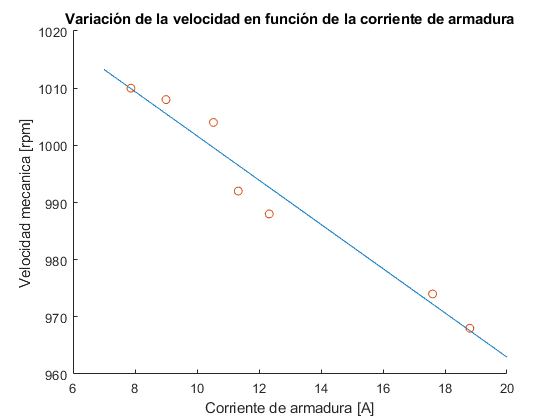
\includegraphics[scale=0.8]{./recursos-Lab6/curvaVelocidadCorriente.png}
		\caption{Curvas Velocidad en función de la corriente}
		\label{fig:CurvaDeVelocidadCorriente}
	\end{figure}

	
	\begin{table}[H]
		\centering
		\caption{Mediciones de porcentaje de regulación}
		\label{Cuadro:Medicion porcentaje de regulacion}
		\begin{tabular}{|c|c|c|}
			\hline
			& pc & sc\\ \hline
			Vshunt(mV)& 32,0 +- 0,1 & 9,7 +- 0,1 \\ \hline
			W (rpm)& 958 +- 2 &1040 +- 2 \\ \hline
			carga(KW)  & 2,8 &0\\ \hline
		\end{tabular}
	\end{table}
 Para determinar el porcentaje de regulación de velocidad de toman los datos de velocidad del Cuadro \ref{Cuadro:Medicion porcentaje de regulacion} a través de la siguiente formula:
 \begin{eqnarray}
  PRN_{\%} =100\%*\frac{n_{sc}-n_{pc}}{n_{pc}}; 
  & \Delta PNR = \frac{1 }{n_{pc}}\cdot \Delta n_{sc}+\frac{n_{sc} }{n_{pc}^2}\cdot \Delta n_{pc}
 \end{eqnarray}
 
Logrando obtener que el porcentaje de regulación de velocidad es de $8,55 \pm 0,43 \%$
\section{Analísis de resultados}
Al comparar los valores de resistencias es notable que la de mayor valor es la referente a la resistencia de campo, siendo el de menor valor la resistencia referente a la de armadura, el valor obtenido de las escobillas según el IEC 34-2 e IEEE std 113-1985 corresponden al tipo metal-grafito, en la Figura \ref{fig:modObtenido} se aprecia el modelo en campo y armadura construidos a partir de lo obtenido.\\

En la prueba de vacío al ajustar una curva polinóica que se adapte con matlab se obtiene la joroba que aparece al inicio de la misma esto sucede en parte a que al tomar los valores descendentes por error se tomaron valores con distancias fuera de lo recomendado, sin embargo se logra apreciar que la curva descendente se encuentra por arriba de la ascendente, debido al flujo remanente lo cual es análogo al ciclo de histéresis dl transformador, que al desenergizar la energía remanente impide que se regrese por la misma curva.\\

    
\end{document}
